\documentclass{standalone}

%----------------------------------------------------------------------------------------------%
%                                 Packages and basic declarations
%----------------------------------------------------------------------------------------------%

\usepackage[utf8]{inputenc}
\usepackage{pgfplots}
\usepackage{tikz}
\usepackage{nicefrac}


%----------------------------------------------------------------------------------------------%
%----------------------------------------------------------------------------------------------%
%                                            DOCUMENT STARTS
%----------------------------------------------------------------------------------------------%
%----------------------------------------------------------------------------------------------%


\begin{document}

\def\markersize{4.5pt}
\def\linewidth{2.5pt}

%Tikz picture starts%

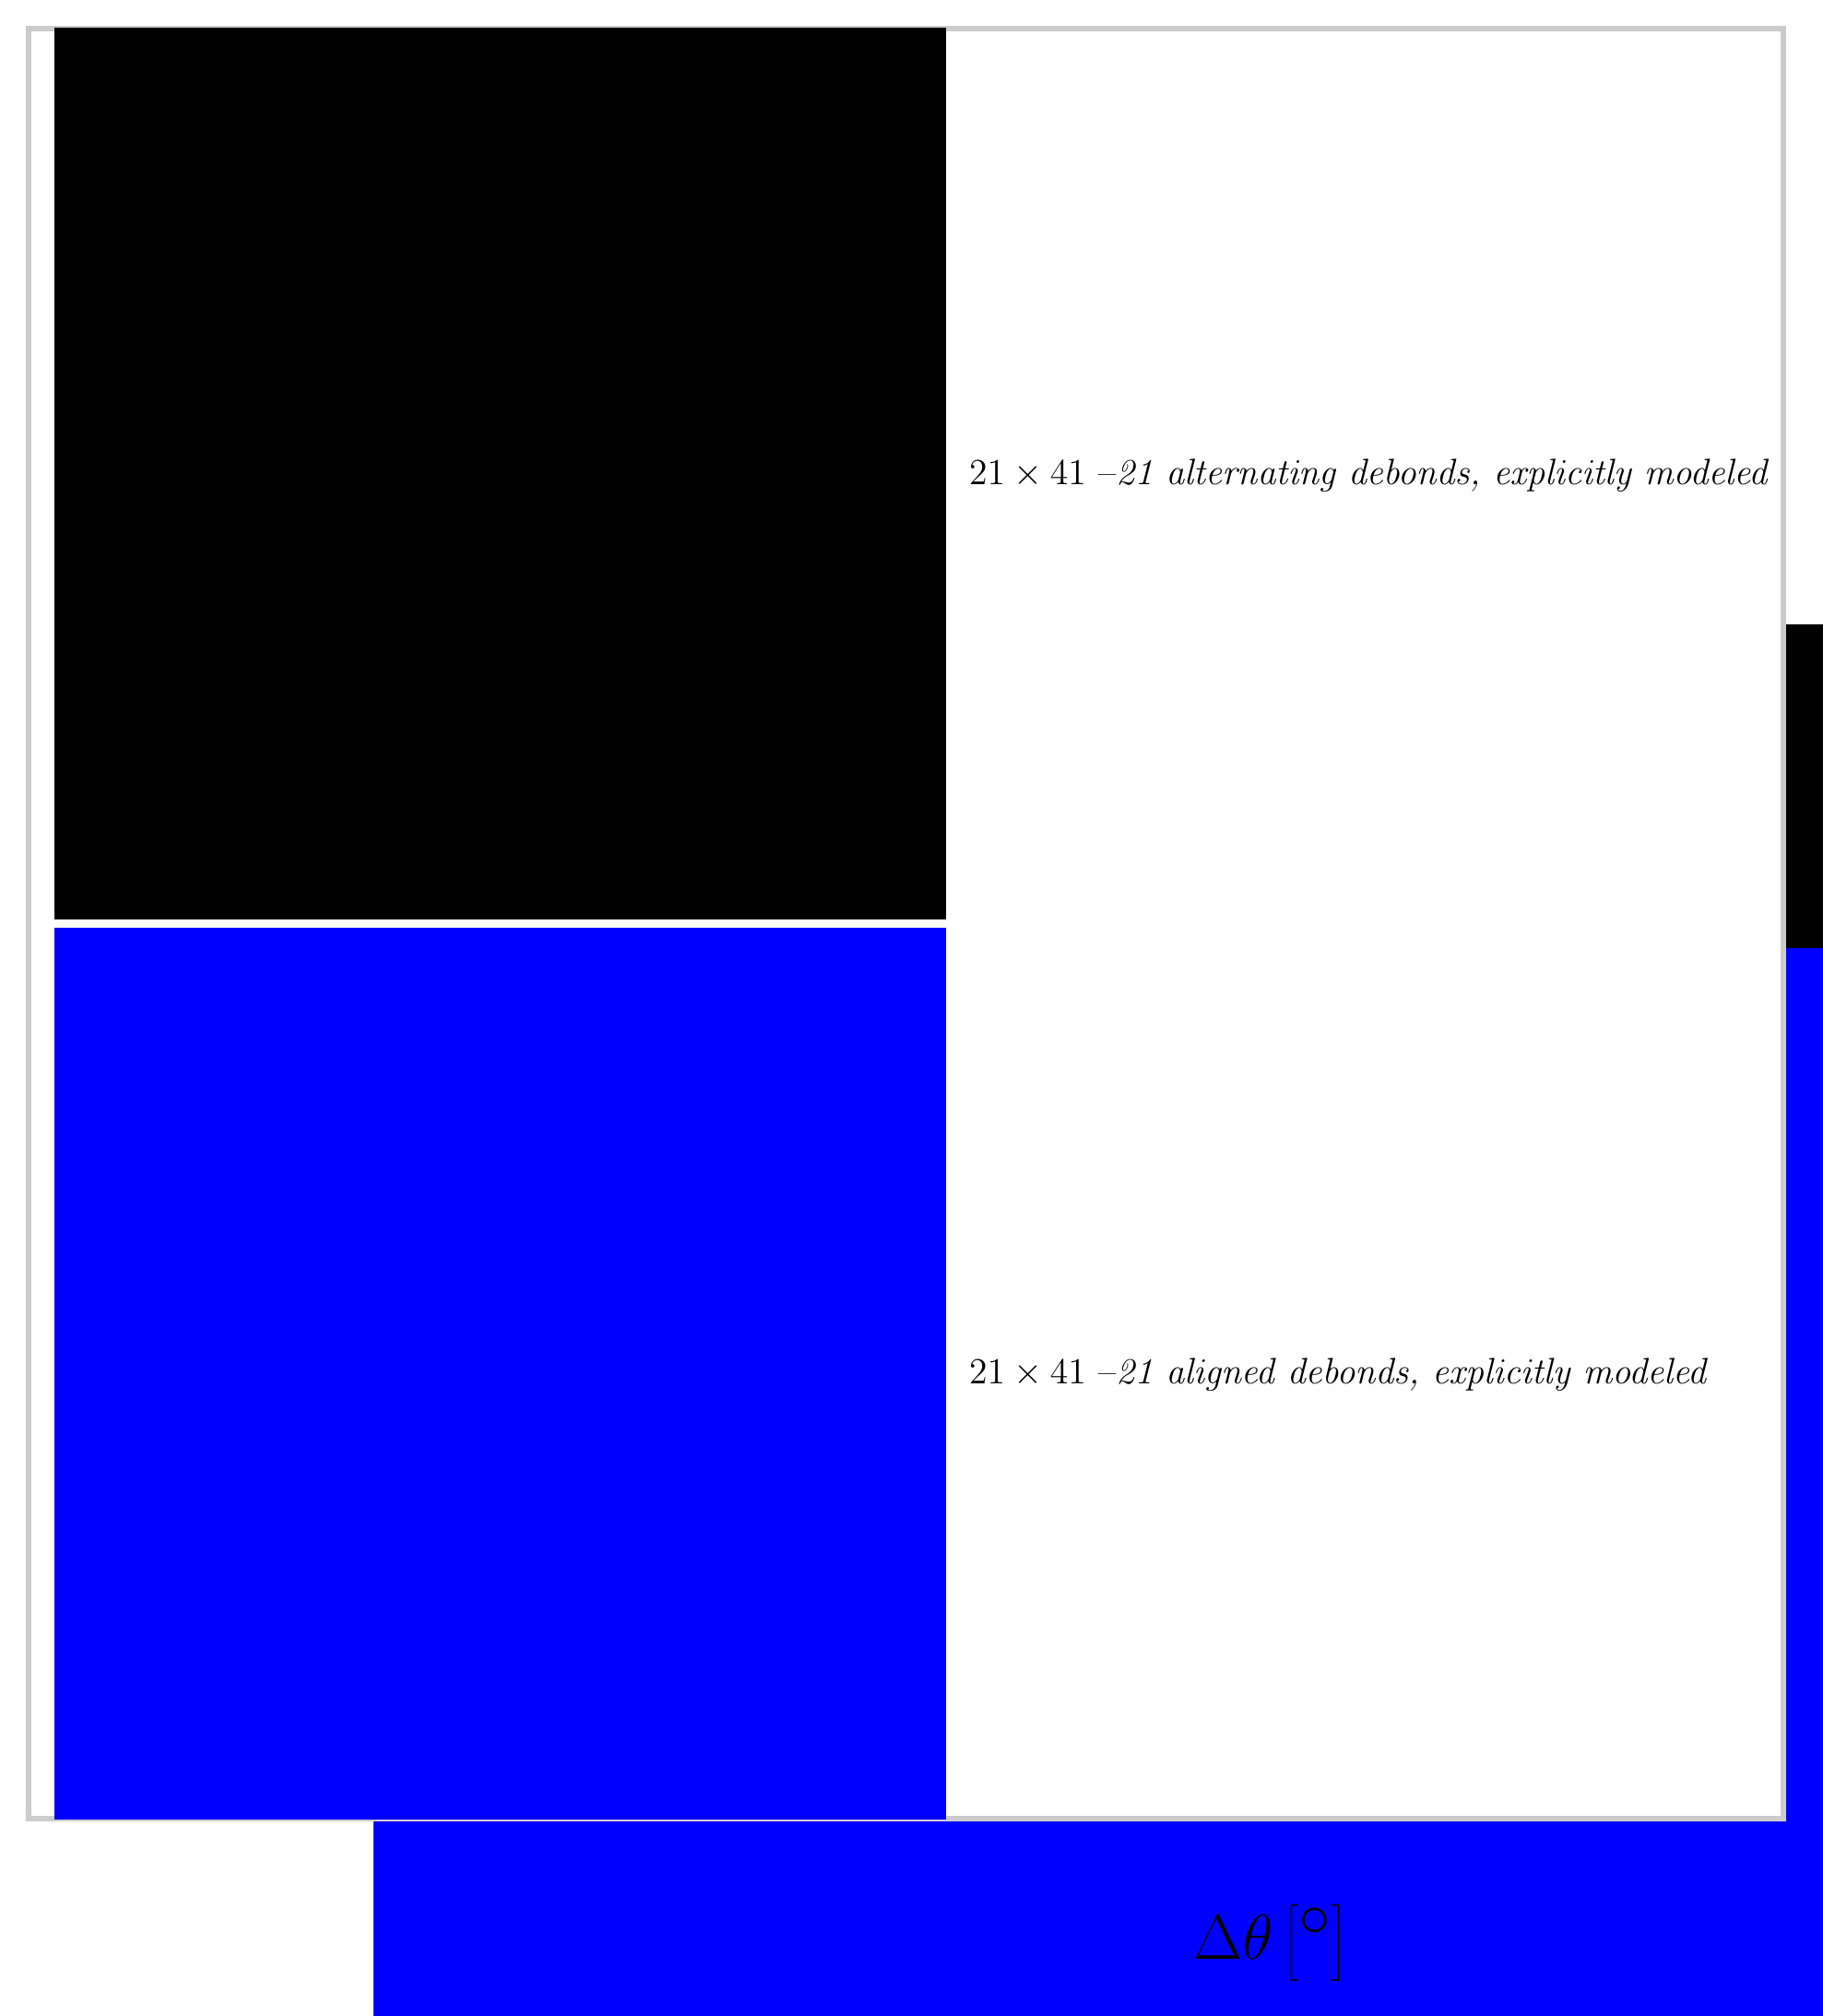
\begin{tikzpicture}

%Tikz axis starts%

\begin{axis}[width=30cm,
% SCALE
scale=0.5,
% STYLE
%title style={font=\fontsize{40}{8}\selectfont},
xlabel style={at={(axis description cs:0.5,-0.025)},anchor=north,font=\fontsize{48}{40}\selectfont},
ylabel style={at={(axis description cs:-0.05,.5)},anchor=south,font=\fontsize{48}{40}\selectfont},
tick align=outside,
tick label style={font=\huge},
legend style={at={(axis description cs:1,1.075)},anchor=east,draw=white!80.0!black,font=\fontsize{15}{14}\selectfont,row sep=7.5pt},
legend image post style={xscale=1.1,yscale=1.1},
legend cell align={left},
clip mode=individual,
% GRID STYLE
xmajorgrids,
x grid style={lightgray!92.026143790849673!black},
ymajorgrids,
y grid style={lightgray!92.026143790849673!black},
line width=0.75mm,
% GRID SIZE
xmin=0.0,
xmax=160.0,
ymin=0.0,
xtick={0.0,10.0,30.0,50.0,70.0,90.0,110.0,130.0,150.0},
% CONTENT
%title={\bf{$\frac{G_{I}}{G_{0}}$ as function of debond's size $\Delta\theta$, in-house VCCT routine}},
xlabel={$\Delta\theta\left[^{\circ}\right]$},
ylabel={$G_{II}\left[\nicefrac{J}{m^{2}}\right]$},
% LEGEND ENTRIES
legend entries={},
]

% asymm - 21x41 - 21 debond expl modeled
\addplot[line width=\linewidth,black,smooth,mark=square*]
table{
10	0.757390072
20	1.757314559
30	2.974771232
40	4.720806908
50	6.328414659
60	8.688349604
70	11.70307237
80	17.09100627
90	14.87164409
100	21.04207754
110	7.985508198
120	4.657742917
130	1.714970454
140	1.127066324
150	0.396694285
};
\addlegendentry{$21\times 41$ --\emph{21 alternating debonds, explicitly modeled}};

% symm - 21x41 - 21 debond expl modeled
\addplot[line width=\linewidth,blue,smooth,mark=square*, mark options={fill=white}]
table{
10	0.752310252
20	1.763303781
30	3.381512999
40	5.570283938
50	7.647319385
60	7.800080835
70	13.53622364
80	16.48155169
90	10.72245358
100	12.55367105
110	6.040989626
120	3.545751301
130	0.789491828
140	0.538696553
150	0.086745537
};
\addlegendentry{$21\times 41$ --\emph{21 aligned debonds, explicitly modeled}};


\end{axis}
%Tikz axis ends%


\end{tikzpicture}
%Tikz picture ends%


\end{document}

%----------------------------------------------------------------------------------------------%
%----------------------------------------------------------------------------------------------%
%                                            DOCUMENT ENDS
%----------------------------------------------------------------------------------------------%
%----------------------------------------------------------------------------------------------%
